\documentclass[10pt, a4paper,english,spanish]{article}

% \usepackage{a4wide}
\parindent = 0 pt
\parskip = 11 pt
\usepackage[width=15.5cm, left=3cm, top=2.5cm, height= 24.5cm]{geometry}
%Margenes de la pagina.  otra opcion, usar \usepackage{a4wide}
%\usepackage[paper=a4paper, left=0.8cm, right=0.8cm, bottom=1.3cm, top=0.9cm]{geometry}
\usepackage{color}
\usepackage{amsmath}
\usepackage{amsfonts}
%este paquete permitcodebe incluir acentos.  Notar que espera un formato ANSI-blah de archivo.  Si en lugar de eso se tiene un utf8 (usual en los linux), entonces usar \usepackage[utf8]{inputenc}
\usepackage[utf8]{inputenc}

\usepackage{tcolorbox}

%Este paquete es para que algunos titulos (como Tabla de Contenidos) esten en castellano
\usepackage[spanish]{babel}

%El siguiente paquete permite escribir la caratula facilmente
\usepackage{caratula}

\usepackage{framed}

\usepackage{graphicx}
\usepackage{float}

\usepackage{algorithm}
\usepackage{algorithmic}
\usepackage{hyperref}

%\usepackage{algpseudocode}

\newcommand{\real}{\mathbb{R}}
\newcommand{\nat}{\mathbb{N}}
\newcommand{\revJ}[1]{{\color{red} #1}}

\newcommand{\refcompleta}[1]{\textbf{Sección \ref{#1} $-$ \nameref{#1}}}


%Datos para la caratula
\materia{Ingeniería de Software II}

\titulo{Trabajo Práctico II}
\subtitulo{Tutor: Javier Martínez Viademonte}

\integrante{Laporte, Matías}{686/09}{matiaslaporte@gmail.com}
\integrante{Salegas, Matías}{750/01}{matias.salegas@gmail.com}
\integrante{Vallejo, Nicolás}{500/10}{nico\_pr08@hotmail.com}
\integrante{Zanitti, Gastón}{58/10}{gzanitti@gmail.com}

\begin{document}

%esto construye la caratula
\maketitle 

\tableofcontents
  \newpage

\section{Introducción}
\indent \indent Esta primera etapa del trabajo consistió en la planificación, utilizando la metodología ágil Scrum, del desarrollo de un simulador de partidos de básquet de fantasía.

\subsection*{User Stories}
Por las características del sistema pedido, donde hay una simulación -que lleva una porción importante de cómputo y representa una etapa del desarrollo bastante \emph{pesada}-, quedaron pocas user stories en total, pues gran parte del sistema se concentra específicamente en ese punto. Esto fue algo que se habló con el tutor y estaba dentro de lo esperable.

Justamente por ser algo que llevaba tanto tiempo, se estuvo en la duda de si convenía o no dividir la \textbf{User Story} correspondiente a la simulación. Una solución propuesta fue especificar en las user stories que una simulación se componía de turnos, éstos de jugadas, y éstas de acciones de los jugadores. Una división de ese modo resultó exagerada, y además iría en contra del principio de independencia para las user stories de \textbf{Scrum}; dado que la simulación debería entrar completa en un único sprint, por lo tanto, se decidió dejarla como una única \textbf{User Story}.


\subsubsection*{Valuación User Stories}
Tanto para la sección de \emph{Business Value} como de \emph{Effort} de cada User Story se decidió realizar poker planning entre los 4 integrantes del grupo. Cuando había discrepancias, se esgrimían los argumentos por los que cada uno había puesto el puntaje correspondiente, de manera de intentar convencer a los otros y así converger los criterios.

\subsection*{Roles}
Otro punto donde hubo ciertas dudas acerca de si se estaba o no en uno de los muchísimos caminos correctos posibles, fue en cuanto a los roles. A primera vista, no parecería haber nadie más que participe del sistema más que el usuario final, a quien llamamos un \emph{participante}. 

Leyendo con un poco más de atención y por cómo se encontraban redactados algunos puntos específicos del enunciado, dejando algunas cosas abiertas con la posibilidad de que sufran modificaciones a futuro, nos pareció propicio considerar un rol de alguien que se encarga de ``mantener'' y administrar el sistema -que seguramente no sea el \emph{dueño}, aunque sí puede que esté dirigido por el mismo-. Ese sería el rol del \emph{administrador}.


\begin{itemize}
\item \textbf{Participante}: es quien se encarga de crear equipos, desafiar a otros participantes y participar de las simulaciones. El \textit{usuario final} del sistema.
\item \textbf{Administrador}: es aquel que actualiza los datos de los jugadores, define las jugadas de cada técnico y las configuraciones de la simulación, tales como la cantidad de turnos de cada una. Es un supervisor del sistema, quien lo regula, el que realiza las acciones para hacerlo más atractivo para los participantes, y más equilibrado.
\end{itemize}

  \newpage
\section{Casos de Uso}
\label{sec:casosdeuso}
A continuación se presenta una lista de los casos de uso que el grupo identificó a partir del enunciado y del QAW provisto. Intentan ser lo suficientemente exhaustivos para cubrir la funcionalidad requerida del sistema a desarrollar.

En conjunto con el análisis de riesgos presentado en una sección subsiguiente, la lista presentada se utilizó para definir el alcance de las iteraciones del plan de proyecto, así como para determinar con mayor nivel de detalle la primer iteración del plan.

Los casos de uso están agrupados aproximadamente según funcionalidad; dado que algunos a veces abarcan más de una de las funcionalidades con las que se los decidió jerarquizarlos a gran escala, realizar una categorización estricta resultaba complejo.


%%%% OBSOLECTOS
%** 40- *consultando datos de jugadores /tecnicos/equipos (participante)
%\item (CU43) - * \textbf{Logueando movimientos de dinero}: (depende de lo que diga Javi) \textbf{---- ??????? -------}
%\item (CU15) -  \textbf{Mostrando desarrollo (log o streaming) de desafío} (sistema -> usuario)
%\item (CU44) - ? \textbf{Mostrando publicidad en la simulación} - ¿es algo que se hace al generar la simulación,  puede ser luego?
%\item (CU37) .- \textbf{Configurando publicidades en simulaciones y en el sitio}:  (representante de empresas (?))
%\item (CU39) - * \textbf{Consultando datos de usuario}: (representantes de empresas(?))
%\item (CU27) - *\textbf{Definiendo reglas de puntajes}:  (administrador)


\subsection{Desafíos}
\subsubsection{Administración de desafíos}
\begin{itemize}
\item (CU3) - 1? \textbf{Definiendo reglas de desafío}: un administrador define las reglas de los partidos de cada liga en base al desempeño de los jugadores reales (cantidad de puntos en el desafío, según acción en la realidad).
\item (CU4) - A2? \textbf{Creando desafío}: un administrador o un participante crea un desafío en el que pueden anotarse una cantidad libre de jugadores.
\item (CU13) - 3? \textbf{Definiendo premios}: el creador de un desafío (un administrador o un participante) elige cómo distribuir los premios o porcentajes del dinero apostado, según las posiciones finales del mismo.
\item (CU26) - * \textbf{Definiendo desafíos interzonales}: un administrador del sistema define desafíos para que participen los mejores jugadores de cada una de las regiones definidas.
\item (CU31) - * \textbf{Configurando visibilidad de los desafíos}: el administrador configura la visibilidad de los desafíos con el fin de que participantes no calificados para participar puedan visualizarlos.
\end{itemize}

\subsubsection{Participación en desafíos}

\begin{itemize}
\item (CU1) - A* \textbf{Eligiendo liga para competir}: un participante elige en qué deporte y liga quiere inscribir a un equipo.
\item (CU5) - A* \textbf{Aceptando desafío}: un participante se anota para participar en uno de los desafíos ya creados.
\item (CU14) - \textbf{Consultando estado (cuenta regresiva, participantes, posiciones) del desafío}: un participante puede consultar datos del desafío donde decidió involucrarse: cuánto falta para que empiece, datos de apuestas, quiénes son los otros participantes, sus posiciones, etc.
\end{itemize}



\subsection{Monetización}
\subsubsection{Dinero real}
\begin{itemize}
\item (CU8) - A* \textbf{Apostando}: un participante apuesta cierta cantidad de dinero en un desafío.
\item (CU10) \textbf{Actualizando datos de medios de pago}: el participante asocia algún medio de pago para poder apostar en los desafíos.
\item (CU33) - * \textbf{Consultando estado de cuenta y movimientos de usuario}: un usuario consulta su estado de cuenta y movimiento. Un administrador puede consultar los datos de cualquier participante del sistema.
\item (CU34) - A* \textbf{Auditando movimientos de dinero}: una entidad gubernamental de control puede auditar los movimientos de todos los usuarios para analizar el movimiento de dinero en el sistema.
\end{itemize}

\subsubsection{Publicidad y marketing}
\begin{itemize}
\item (CU16) - * \textbf{Configurando publicidad en el sitio y simulaciones}: un representante de empresa sponsor del proyecto puede acceder a una interfaz desde donde se configura la publicidad que se muestra en el sitio y las simulaciones a los participantes.
\item (CU38) -* \textbf{Configurando publicidad y ads en transmisiones}: un representante de empresa dueña de los derechos de televisación puede modificar las publicidades y ads que se muestran en las transmisiones de los partidos a los participantes.
\item (CU17) - \textbf{Acceder a datos de preferencia/comportamiento de usuarios}: un administrador o un representante de empresa accede a estadísticas que permiten obtener insights de negocio, en base al comportamiento y las opciones más utilizadas por los usuarios.
\end{itemize}

\subsection{Registro, Autenticación y Datos de usuario}

\subsubsection{Cuentas de usuarios}
\begin{itemize}
\item (CU9) - * \textbf{Creando cuenta de usuario}: un participante se registra en el sistema para poder participar de los desafíos
\item (CU12)- * \textbf{Consultando cuenta de usuario}: un participante o administrador consulta los datos con los que se dio de alta el usuario en el sistema.
\item (CU41) - *\textbf{Desactivando cuenta}: un participante o representante de una organización de protección al consumidor puede desactivar una cuenta temporalmente para ayudar a adictos al juego a no tener recaídas.
\item (CU42) - *\textbf{Reactivando cuenta}: un participante puede reactivar su cuenta luego del tiempo establecido en la desactivación.
\item (CU28) - * \textbf{Consultando dashboard regional o global}: un administrador o representante de empresa sponsor del proyecto puede acceder a un dashboard con el estado de cuenta en tiempo real del sitio para cada una de las regiones y niveles y de cualquier grupo de participantes.
\end{itemize}

\subsubsection{Ranking y puntajes}

\begin{itemize}
\item (CU29) -* \textbf{Consultando ranking de jugadores}: un participante puede consultar el ranking de jugadores en cualquier momento y ver su posición en el mismo.
\item (CU32) - * \textbf{Reiniciando el ranking de jugadores}: un administrador reinicia el ranking actual de jugadores, volviendo a todos a la situacion inicial para dar inicio a una nueva temporada.
\end{itemize}


\subsection{Social}
\begin{itemize}
\item (CU6) - * \textbf{Participando del chat general}: un participante envía un mensaje al chat general para que lo vean todos los demás participantes del desafío.
\item (CU7) -.* \textbf{Participando de chat privado}: un participante envía un mensaje privado a otro participante y solo éste puede verlo.
\item (CU23)- ? \textbf{Recolectando opiniones de redes sociales y chats}: se recolectan opiniones de las redes sociales y los chats generales y privados del sistema para afectar los resultados de las simulaciones.
\item (CU24)- * \textbf{Definiendo impacto de opiniones}: un administrador define de qué forma los comentarios obtenidos en las redes sociales impactan en el resultado de los desafíos o en la performance de los jugadores.
\end{itemize}

\subsection{Simulaciones}
\subsubsection{Ejecución}
\begin{itemize}
\item (CU18) - \textbf{Definiendo reglas de simulación}: un administrador modifica las reglas de las simulaciones de los deportes basándose en los comentarios recibidos por el comité de expertos de cada uno de ellos.
\item (CU2) - * \textbf{Obteniendo datos en tiempo real}: se obtienen en tiempo real, mediante empresas proveedoras, datos de los jugadores y del desarrollo de los partidos de las APIs provistas para mantenerlos actualizados. 
\end{itemize}


\subsubsection{Visualización}
\begin{itemize}
\item (CU19) - ? \textbf{Mostrando detalle minuto a minuto de la simulación}: los participantes pueden ver un detalle minuto a minuto de las simulaciones.
\item (CU20) - * \textbf{Observando evento global / continental}: un participante puede acceder a desafíos donde no puede participar en modo espectador, según las reglas dispuestas por los administradores.
\item (CU21) - * \textbf{Mostrando simulación gráfica (motor 2d, motor 3d)}: se genera una simulación gráfica que se muestra al usuario para que pueda disfrutar del desafío de otra manera.
\item (CU22) - * \textbf{Observando la transmisión de un partido de liga}: los participantes pueden ver la transmisión de los partidos en los desafíos en modo \emph{liga de fantasía tradicional}.
\item (CU35) - A* \textbf{Auditando simulaciones}: una entidad gubernamental de control puede auditar las simulaciones para corroborar que se correspondan con los resultados obtenidos y los desafíos pagados.
\end{itemize}


\subsection{Regionalización}
\begin{itemize}
\item (CU25) - * \textbf{Definiendo regiones de la plataforma}: un administrador de la plataforma define regiones y niveles para los mismos, con el fin de regionalizar la plataforma y facilitar la comunicación entre los participantes, la integración con los bancos, el cumplimiento de legislación vigente en los distintos países, etc.
\item (CU36) - * \textbf{Definiendo restricciones por zona}: un administrador define qué deportes están disponibles para cada una de las zonas y si es posible apostar con dinero real, etc. Involucra también definir si el sitio es accesible en cada país.
\end{itemize}







  \newpage
\section{Riesgos}
Análisis de Riesgos

Riesgo 1

Descripción: El experto en redes de la empresa proveedora de infraestructura exige de manera prioritario para el próximo mes el diagrama híbrido  c&c/allocation>deployment
que detalla el manejo del streaming de partidos/simulaciones a todas las regiones en el caso de un evento global o continental. Dado que los mientras del equipo carecen del conocimiento necesario en el tema, es posible que no se llegue a cumplir el plazo.
Probabilidad: Alta
Impacto: Alto
Exposición: Alta
Mitigación : Priorizar el desarrollo del mecanismo de streaming, introduciéndolo en la primera iteración.
Plan de Contingencia : Contratar los servicios de una empresa especializada en el tema
que se encargue del desarrollo.

Riesgo 2
Descripción : Los datos correspondientes a los medios de pago, es decir, tarjetas de crédito
y números de cuentas bancarias, deben almacenarse de forma segura y confidencial  a modo de evitar ataques destinados al robo de información. Dado la sensibilidad de la información no sería totalmente inesperado ser objeto de un ataque.
Probabilidad : Baja
Impacto: Alto
Exposición : Media
Mitigación : Encriptar los datos de los medios de pago de los participantes y de los canales de comunicación de la plataforma. Además, agregar mecanismos verificación de la identidad de los participantes:
Plan de Contingencia: En caso de detección de ataque, aislar los servidores donde se guardan los datos, desconectándolos del sistema, hasta tanto no se haya resuelto la intromisión.


Riesgo 3
Descripción : Es importante que el sistema esté disponible la mayor cantidad del tiempo posible.Hay que tener especial cuidado ya que se rumorea que los servidores de la empresa proveedora de servicios se caen sin previo aviso, y la caída del sistema implicaría
pérdida de dinero.
Probabilidad: Media
Impacto: Alto
Exposición: Alta
Mitigación: Definir un mecanismo de redundancia de servidores. Cualquier acción como la carga de datos por parte del usuario podría hacerse de forma offline y sincronizarse con el sistema una vez resuelto el problema de conexión.
Plan de Contingencia: Contratar otra empresa proveedora de servicios, ya sea como respaldo o reemplazando a la actual como proveedora principal.


Riesgo 4: 
Descripción: La trasmisión de la partidos debe hacerse con la mejor calidad posible y sin cortes ya que no hacerlo impediría cumplir con el estándar de calidad que exigen las ligas para mantener los derechos de transmisión.
Probabilidad: Media
Impacto : Alto
Exposición: Alta
Mitigación: Desarrollar un mecanismo de bitrate variable para el streaming de video, dependiente de las características de la conexión de los usuarios.
Plan de Contingencia: Tercerizar el streaming a través de una plataforma con harta experiencia en el tema, como podría ser Youtube.


Riesgo 5

Descripción: Dado el método de definición de las simulaciones y de los desafíos, es de vital
importancia que los datos provenientes de las empresas proveedoras de los resultados minuto a minuto de los encuentros sean totalmente confiables y representaciones correctas de los desarrollos de los encuentros de la realidad. La inconsistencia de estos datos puede traer como consecuencia resultados incorrectos en los desafíos y el pago erróneo de premios.
Probabilidad: Baja
Impacto : Alto
Exposición: Media
Mitigación: Diseñar un mecanismo de transmisión de los datos de las empresas proveedoras de los resultados minuto a minuto que sea confiable, íntegro y seguro.
Además, desarrollar un algoritmo que se base en contrastar los resultados provistos por más de una empresa para el mismo encuentro con el fin de detectar inconsistencias.
Plan de Contingencia: Deshabilitar el minuto a minuto en el momento en el que se desconfíe de los datos, hasta tanto no se solucione el tema. En tal situación, los resultados de los desafíos se definirán basados en los datos que se puedan obtener luego de los encuentros,en cuyo caso pueden validarse de manera más fácil.


Riesgo 6

Descripción: Es importante proveer el acceso correspondiente tanto a la plataforma en su totalidad como a sus diferentes secciones de acuerdo a la legislación vigente de cada país. No hacerlo podría incurrir en la comisión de delitos.
Probabilidad: Media
Impacto: Alto
Exposición: Alta
Mitigación : Diseñar e implementar un mecanismo lo suficientemente elástico para configurar el acceso a las distintas modalidades de la plataforma. Mantener un equipo que periódicamente se informa acerca de las distintas legislaciones de cada país.
Plan de Contingencia: En caso de poseer dudas con respecto a la legalidad del funcionamiento de la plataforma en un país, impedir el ingreso al sitio hasta tanto se haya validado y consultado sobre las normativas, evitando así potenciales actos ilegales.


Riesgo 7
Descripción : Es menester mantener la transparencia de los módulos de simulaciones, a modo de evitar la interferencia de agentes externos en su ejecución. Un ataque al sistema podría involucrar la alteración del módulo de simulación, provocando la existencia de resultados adulterados.
Probabilidad: Baja
Impacto : Medio
Exposición: Baja
Mitigación: Desarrollar mecanismos de testeo de la simulación en servidores testigos donde los resultados se sepan de antemano. Diseñar un mecanismo que ante inconsistencias realice un deploy de una versión válida del módulo simulador.
Plan de Contingencia: Prohibir la realización de simulaciones hasta tanto se verifique el correcto funcionamiento.


Riesgo 8
Descripción: Los stakeholders quieren tener confianza en que vamos a ser capaces de guardar los datos de tarjetas de crédito, como hacen otros sitios exitosos. Si no nos mostramos seguros, pueden darle (parte de) el proyecto a otro equipo de desarrollo.
Probabilidad: Baja.
Impacto: Alto.
Exposición: Media.
Mitigación: Mostrar ejemplos de trabajos nuestros en los que no tuvimos esos problemas.
Plan de contingencia: ???

Riesgo 9
Descripción: Los distintos sponsors tienen intereses distintos, algunos de ellos contrapuestos. Por ejemplo, las empresas televisivas están en contra de las simulaciones. Puede ser que parte del proyecto cambie o se cancele.
Probabilidad: Baja.
Impacto: Medio.
Exposición: Baja.
Mitigación: Mantener reuniones periódicas con los sponsors y convencerlos de que ambas funcionalidades son buenas para el proyecto.
Plan de contingencia: Diseñar una arquitectura flexible, que se adapte a los cambios.

Riesgo 10
Descripción: Hay otros aspectos todavía no definidos y que no dependen de nosotros. Por ejemplo, en qué países se va a usar cada parte del juego. Puede pasar que cambien los requerimientos después de que empezamos.
Probabilidad: Media.
Impacto: Medio.
Exposición: Media.
Mitigación: Exigir a los stakeholders que tomen decisiones y las comuniquen lo antes posible.
Plan de contingencia: Diseñar una arquitectura flexible, que se adapte a los cambios.

Riesgo 11
Descripción: El equipo nunca trabajó con esta metodología. Puede pasar que la adaptación lleve más tiempo de lo planeado.
Probabilidad: Media.
Impacto: Medio.
Exposición: Alta.
Mitigación: Consultas periódicas con un experto.
Plan de contingencia: Aumentar las consultas al experto.

Riesgo 12
Descripción: El equipo tuvo problemas de comunicación antes. Si se repiten, pueden afectar todo el trabajo. Trabajamos mucho de manera remota y tenemos distintos horarios.
Probabilidad: Media.
Impacto: Alto.
Exposición: Alta.
Mitigación: Reuniones periódicas e intercambio de mails diarios.
Plan de contingencia: Reuniones de emergencia y buscar vías de comunicación instantáneas, como chats y teléfono.

Riesgo 13
Descripción: Es probable que la planificación no sea exacta, tanto en las tareas como en los tiempos pensados para cada una.
Probabilidad: Alta.
Impacto: Medio.
Exposición: Alta.
Mitigación: Sobreestimar los tiempos y las dificultades.
Plan de contingencia: Evaluar y adaptar la planificación luego de la primera iteración.


  \newpage
\section{Plan de Proyecto}
\label{sec:planificacion}
\subsection{Iteraciones}
Las iteraciones tienen una duración aproximada de 3 semanas (15 días hábiles). Teniendo en cuenta que los recursos asignados son 4 arquitectos de software/programadores trabajando de modo part-time (6 horas), se estiman unas 360hrs. aproximadas por iteración.

Nuestra decisión sobre la conformación de las iteraciones -en cuanto a los casos de uso- se rigió por varios factores: 
\begin{itemize}
\item Se tuvieron en cuenta las necesidades extraídas del QAW con los stakeholders
\item Se trató de agrupar a los casos de uso por su temática, prefiriendo en caso de ser posible juntar dentro de una misma iteración los casos de uso que se relacionan con funcionalidades similares.
\item Otro factor que se tuvo en cuenta a la hora de definir el orden de las iteraciones, fueron los riesgos detectados y analizados en la sección de Análisis de Riesgos (\ref{sec:riesgos}).
\item También se consideró la prioridad de la funcionalidades referidas en los casos de uso, intentando en lo posible desarrollar antes las más importantes para el negocio.
\end{itemize}

La primera iteración quedó expresamente definida por el QAW y el análisis de riesgo, factores a los que se les dio mayor prioridad. 
Del análisis de riesgo, y dado el factor prioritario que tiene la disponibilidad del sistema, se extrajo que la parte más conflictiva ocurre a la hora de transmitir los desafíos (especialmente para los eventos globales), así como al mostrar correctamente las simulaciones.

El siguiente punto en cuanto a nivel de riesgo, fue lo concerniente a la seguridad, integridad y transparencia de la transmisión de los datos de pago y movimientos de dinero, y las transmisiones de datos usadas para definir los resultados de los partidos de la realidad y minuto a minuto de las simulaciones. Decidimos encarar esto en la segunda iteración del proyecto.

Otro foco de preocupación y de vital importancia para el proyecto, es su alcance y monetización. Por esa razón, se decidió trabajar en lo que respecta a las publicidades del sitio, simulaciones y transmisiones (y el uso de los datos de comportamiento de usuarios), además de la regionalización del sistema (con todas las reglas y restricciones que eso conlleva) en la tercer iteración.

El manejo administrativo de las cuentas de los usuarios, y el aspecto \emph{social} (chat, utilización de las opiniones vertidas en redes sociales, etc.), consideradas cuestiones de menor complejidad, se decidieron enfrentar en la cuarta iteración.

Decidimos dedicarnos en la quinta iteración a todo lo referido a los desafíos, su creación, configuración, definición de reglas y de los premios. En la sexta iteración, nos encargaremos de lo que concierne a los rankings de los jugadores globales, regionales, etc. Como los casos de uso de estas dos iteraciones tienen un menor riesgo y complejidad que los anteriores, consideramos que estas dos fases son de construcción, ya que se trabajará bastante en lo implementativo y poco en el análisis/diseño.



\subsubsection{I01 - Primera Iteración (Elaboración)}
\begin{itemize}
\item (CU19) Mostrando detalle minuto a minuto de la simulación
\item (CU2)  Obteniendo datos en tiempo real
\item (CU21) Mostrando simulación gráfica
\item (CU22) Observando la transmisión de un partido de liga
\item (CU20) Observando evento global/continental
%\item CU15) Mostrando desarrollo (log o streaming) de desafío} (sistema -> usuario)
\end{itemize}

\subsubsection{I02 - Segunda iteración (Elaboración)} 
\begin{itemize}
\item (CU9) Creando cuenta de usuario
\item (CU10) Actualizando datos de medios de pago
\item (CU34) Auditando movimientos de dinero
\item (CU33) Consultando estado de cuenta y movimientos de usuario
\item (CU35) Auditando simulaciones
\item (CU8) Apostando
%\item CU43) Logueando movimientos de dinero}: (depende de lo que diga Javi)
\end{itemize}


\subsubsection{I03 - Tercera Iteración (Elaboración)}
\begin{itemize}
\item (CU36) Definiendo restricciones por zona
\item (CU25) Definiendo regiones de la plataforma
\item (CU18) Definiendo reglas de simulación
\item (CU38) Configurando publicidad y ads en transmisiones
\item (CU16) Configurando publicidad en el sitio y simulaciones
\item (CU17) Acceder a datos de preferencia/comportamiento de usuarios
%\item (CU44) Mostrando publicidad en la simulación} - ¿es algo que se hace al generar la simulación,  puede ser luego?
%\item (CU37) Configurando publicidades en simulaciones y en el sitio}:  (representante de empresas (?))
%\item (CU39) Consultando datos de usuario}: (representantes de empresas(?))
\end{itemize}


\subsubsection{I04 - Cuarta Iteración (Elaboración)}
\begin{itemize}
\item (CU6) Participando del chat general
\item (CU7) Participando de chat privado
\item (CU12) Consultando cuenta de usuario
\item (CU41) Desactivando cuenta
\item (CU42) Reactivando cuenta
\item (CU23) Recolectando opiniones de redes sociales y chats
\item (CU24) Definiendo impacto de opiniones
%4- consultando datos de jugadores /técnicos /equipos (participante)
\end{itemize}

\subsubsection{I05 - Quinta Iteración (Construcción)}
\begin{itemize}
\item (CU1) Eligiendo liga para competir
\item (CU3) Definiendo reglas de desafío
\item (CU4) Creando desafío
\item (CU5) Aceptando desafío
\item (CU14) Consultando estado (cuenta regresiva, participantes, posiciones) del desafío
\item (CU13) Definiendo premios
\end{itemize}

\subsubsection{I06 - Sexta Iteración (Construcción)}
\begin{itemize}
\item (CU28) Consultando dashboard regional o global
\item (CU29) Consultando ranking de jugadores
\item (CU32) Reiniciando el ranking de jugadores
\item (CU26) Definiendo desafíos interzonales
\item (CU31) Configurando visibilidad de los desafíos
%6 -  definiendo reglas de puntajes (administrador)
\end{itemize}


\subsection{Primera iteración (I01) en detalle}
\label{subsec:primeraiteracion}
En esta sección se realiza un detalle de las tareas que se consideran necesarias realizar en la primer iteración, junto a las horas hombres esperadas. Dado que ya se realizó un reconocimiento, priorización, y estimación de tiempo de los casos de uso, además del análisis de riesgo, no serán tareas prioritarias ni de mucha intensidad en esta etapa, sino que se utilizarán para poder corregir detalles de las futuras iteraciones.

Algunas de las tareas (por ejemplo I01T01, I01T02, I01T03) que no se corresponden directamente con un caso de uso, tienen como objetivo la mitigación de los riesgos analizados (\ref{sec:riesgos}).

\begin{itemize}
\item \underline{I01T01} - Reunión semanal breve con stakeholders para asegurarse que los requerimientos estén actualizados: \textbf{10hs}.
  \begin{itemize}
    \item \underline{I01T01ST01} - Reunión la primer semana: 4hs.
    \item \underline{I01T01ST02} - Reunión la segunda semana: 3hs.
    \item \underline{I01T01ST03} - Reunión la tercer semana: 3hs.
  \end{itemize}
\hfill

\item \underline{I01T02} - Reunión cada 3 días hábiles del equipo para evitar problemas de comunicación como en el pasado: \textbf{10hs}.
  \begin{itemize}
    \item \underline{I01T02ST01} - Primera reunión: 2hs.
    \item \underline{I01T02ST02} - Segunda reunión: 2hs.
    \item \underline{I01T02ST03} - Tercer reunión: 2hs.
    \item \underline{I01T02ST04} - Cuarta reunión: 2hs.
    \item \underline{I01T02ST05} - Quinta reunión: 2hs.
  \end{itemize}
\hfill

\item \underline{I01T03} - Reunión semanal de consulta con experto en metodología UP: \textbf{8hs}.
  \begin{itemize}
    \item \underline{I01T03ST01} - Reunión la primer semana: 3hs.
    \item \underline{I01T03ST02} - Reunión la segunda semana: 2hs.
    \item \underline{I01T03ST03} - Reunión la tercer semana: 2hs.
  \end{itemize}
\hfill

\item \underline{I01T04} - Identificación y descripción de los atributos de calidad del sistema: \textbf{40hs}.
  \begin{itemize}
    \item \underline{I01T04ST01} - Cotejamiento de los atributos definidos por stakeholders en QAW y relación con los casos de uso definidos: 16hrs.
    \item \underline{I01T04ST02} - Descripción de escenarios de atributos de calidad: 20hs.
    \item \underline{I01T04ST03} - Verificación de la documentación escrita: 4hs.
  \end{itemize}
\hfill
  
\item \underline{I01T05} - Diseño de la arquitectura del sistema: \textbf{60hs}.
  \begin{itemize}
    \item \underline{I01T05ST01} - Analizar los escenarios descritos en I01T04 e identificar drivers de arquitectura: 8hs. 
    \item \underline{I01T05ST02} - Estudiar y elegir patrones arquitectónicos que satisfagan los drivers identificados: 12hs.
    \item \underline{I01T05ST03} - Verificar y refinar los casos de usos y los escenarios: 10hs.
    \item \underline{I01T05ST04} - Iterar: 30hs.
   \end{itemize}
\hfill

\item \underline{I01T06} - Realización de las tareas del (CU2)  Obteniendo datos en tiempo real: \textbf{40hs}.
  \begin{itemize}
    \item \underline{I01T06ST01} - Reunirse con empresas que provean datos en tiempo real de la evolución de los partidos y contratar alguna: 12hs.
    \item \underline{I01T06ST02} - Reunirse con la empresa contratada y obtener documentación técnica sobre la API que proveen: 2hs.
    \item \underline{I01T06ST03} - Investigar la API y analizar qué datos podemos usar como input en nuestro sistema: 6hs.
    \item \underline{I01T06ST04} - Adaptar nuestro sistema para que los desafíos en modo \emph{Liga de fantasía} utilicen los datos obtenidos a través de la api: 10hs.
    \item \underline{I01T06ST05} - Realizar algunos desafíos y verificar que los resultados de los puntajes se condigan con lo que ocurrió en los partidos reales: 6hs.
    \item \underline{I01T06ST06} - Corregir potenciales errores: 4hs.
  \end{itemize}
\hfill

\item \underline{I01T07} - Realización de las tareas del (CU19) Mostrando detalle minuto a minuto de la simulación: \textbf{40hs}.
  \begin{itemize}
    \item \underline{I01T07ST01} - Investigar el log del desarrollo anterior, cómo se genera y la calidad de la salida: 4hs.
    \item \underline{I01T07ST02} - Reunirse con las empresas desarrolladoras de los dos motoroes gráficos y averiguar qué tipo de entrada necesitan: 6hs.
    \item \underline{I01T07ST03} - Comparar el log actual con el que se necesita y definir qué es lo que falta agregar: 4hs.
    \item \underline{I01T07ST04} - Agregar el detalle necesario al log de salida para cumplir con lo requerido por las empresas: 10hs.
    \item \underline{I01T07ST05} - Ajustar la velocidad de salida del log para que no sea instantánea, sino minuto a minuto, y respete la nueva duración (similar a la de un partido real) de las simulaciones: 5hs.
    \item \underline{I01T07ST06} - Realizar algunas ejecuciones de prueba y obtener logs de salida de ejemplo: 4hs.
    \item \underline{I01T07ST07} - Corroborar con empresas proveedoras que el detalle del log obtenido sea el correcto: 2hs.    
    \item \underline{I01T07ST08} - Corregir potenciales errores: 5hs.
  \end{itemize}
\hfill

\item \underline{I01T08} - Realización de las tareas del (CU21) Mostrando simulación gráfica: \textbf{50hs}.
  \begin{itemize}
    \item \underline{I01T08ST01} - Reunirse con empresa de motor 3D y discutir sobre los requerimientos técnicos para la transmisión de video en dispositivos no soportados por el motor gráfico: 10hs.
    \item \underline{I01T08ST02} - Obtener varios logs minuto a minuto de prueba y utilizarlos como entrada para los distintos motores gráficos. Comparar que el resultado gráfico (según limitaciones de cada motor) de los partidos sea el mismo y no haya diferencias: 20hs.
    \item \underline{I01T08ST03} - Probar los motores en distintos dispositivos y obtener los requerimientos mínimos y recomendados de hardware para poder informar a los participantes: 15hs.
    \item \underline{I01T08ST04} - Escribir documentación sobre los distintos motores, obtener screenshots para poder publicar en el home del producto como ejemplo de jugabilidad: 5hs.
  \end{itemize}
\hfill


\item \underline{I01T09} - Realización de las tareas del (CU22) Observando la transmisión de un partido de liga: \textbf{65hs}.
  \begin{itemize}
    \item \underline{I01T09ST01} - Reunirse con la empresa dueña de los derechos de televisión y la empresa proveedora de infraestructura para definir sus requerimientos, necesidades, y llegar a acuerdos comunes en los puntos álgidos: 10hs.
    \item \underline{I01T09ST02} - Reunirse con la empresa proveedora de infraestructura de redes para definir la arquitectura de hardware a utilizar para el sistema: 8hs.
    \item \underline{I01T09ST03} - Implementar la solución de hardware convenida con la empresa proveedora de infraestructura de redes: 16hs.
    \item \underline{I01T09ST04} - Realizar pruebas internas de transmisión en vivo de eventos con diferentes cargas en los servidores y desde distintas regiones: 16hs.
    \item \underline{I01T09ST05} - Dar feedback a la empresa proveedora de infraestructura y ver, de ser necesario, cómo mejorar el rendimiento: 10hs.
    \item \underline{I01T09ST06} - Mostrarle a la empresa dueña de los derechos de televisión el funcionamiento del sistema y verificar que cumpla con sus requerimientos: 5hs.
  \end{itemize}
\hfill

\item \underline{I01T10} - Realización de las tareas del (CU20) Observando evento global/continental: \textbf{hs}.
  \begin{itemize}
    \item \underline{I01T10ST01} - : XXhs.
    \item \underline{I01T10ST02} - : XXhs.
    \item \underline{I01T10ST03} - : XXhs.
    \item \underline{I01T10ST04} - : XXhs.
  \end{itemize}
\hfill

La suma de las tareas para la primer iteración da ???hs. Habiendo calculado una iteración ideal de 360hs. nos da cierto margen como para poder afrontar tareas urgentes o no previstas.

\subsection{Diagrama de Gantt}
  
\end{itemize}

  \newpage
\section{Atributos de calidad}

En esta sección se presentan los atributos de calidad identificados en el TP (ordenados según la prioridad definida por los \emph{stakeholders} en el \emph{Quality Attribute Workshop}), junto a sus respectivos escenarios.

% \begin{center}
%   \begin{tabular}{| l | p{10cm} | }
%     \hline
% 	\textbf{Descripción} & UNA DESCRIPCION\\  \hline
% 	\textbf{Fuente} & UNA FUENTE\\  \hline
% 	\textbf{Estímulo} & UN ESTIMULO\\  \hline
% 	\textbf{Entorno} & UN ENTORNO\\  \hline
% 	\textbf{Artefacto} & UN ARTEFACTO\\  \hline
% 	\textbf{Respuesta} & UNA RESPUESTA\\  \hline
% 	\textbf{Medición} & UNA MEDICION\\  \hline
%   \end{tabular}
% \end{center} 

\subsection{Disponibilidad}

\subsubsection*{Motivación}
\begin{itemize}
\item El sistema tiene que estar andando todo el tiempo.
\item Cantidad de usuarios limitada - máxima por servidor
\item Múltiples nodos distribuidos de pocos usuarios cada uno.
\item Los partidos streameados deben darse en excelente calidad sin cortes.
\item Cuando ninguno de los motores gráficos se encuentra disponible, debe usarse el streaming del engine 3D.
\item Debe esforzarse por respetar a los países en los que la legislación vigente no permite directamente que se ingrese al sitio.
\item Debe ser fácil desactivar una cuenta por un tiempo, sin poder reactivarla, tanto para usuarios adictos en recuperación como para usuarios de países en los que no está disponible el sitio.
\end{itemize}

\subsubsection*{Escenarios}
\begin{center}
  \begin{tabular}{| l | p{10cm} | }
    \hline
	\textbf{Descripción} & En caso de saturación de un nodo, deben direccionarse nuevas conexiones a otro nodo.\\  \hline
	\textbf{Fuente} & Usuario\\ \hline
	\textbf{Estímulo} & Se realiza un request al sistema.\\  \hline
	\textbf{Entorno} & Nodo saturado\\  \hline
	\textbf{Artefacto} & Nodo del sistema\\  \hline
	\textbf{Respuesta} & Se selecciona un nuevo nodo regional y se continúa el servicio mediante una conexión con él.\\  \hline
	\textbf{Medición} & El 99.99 \% de las nuevas conexiones se realizan sin inconveniente alguno y de forma transparente al usuario.\\  \hline
  \end{tabular}
\end{center} 


\begin{center}
  \begin{tabular}{| l | p{10cm} | }
    \hline
	\textbf{Descripción} & Los streamings de partidos se realizan con la menor cantidad de cortes posibles.\\  \hline
	\textbf{Fuente} & Usuario\\  \hline
	\textbf{Estímulo} & Solicita ver el streaming de un partido\\  \hline
	\textbf{Entorno} & Normal\\  \hline
	\textbf{Artefacto} & Generador gráfico\\  \hline
	\textbf{Respuesta} & Se realizan los cálculos pertinentes para determinar el ancho de banda del usuario y se comienza el streaming con la calidad determinada.\\  \hline
	\textbf{Medición} & Se produce a lo sumo un corte con duración menor a 5 segundos por transmisión.\\  \hline
  \end{tabular}
\end{center}

\begin{center}
  \begin{tabular}{| l | p{10cm} | }
    \hline
	\textbf{Descripción} & Si los motores gráficos para una simulación no están disponibles, debe realizarse un streaming del engine 3D para la simulación. \\  \hline
	\textbf{Fuente} & Usuario \\  \hline
	\textbf{Estímulo} & Intenta observar una simulación\\  \hline
	\textbf{Entorno} & Motores gráficos del dispositivo no disponibles.\\  \hline
	\textbf{Artefacto} & Generador gráfico\\  \hline
	\textbf{Respuesta} & Ante la detección de la imposibilidad de utilizar los motores gráficos en el dispositivo, se activa el streaming del engine 3D de la simulación.\\  \hline
	\textbf{Medición} & Se trasmite la simulación 3D sin inconvenientes en el 99\% de los casos.\\  \hline
  \end{tabular}
\end{center}  

\begin{center}
  \begin{tabular}{| l | p{10cm} | }
    \hline
	\textbf{Descripción} & Si se detecta que los motores gráficos vuelven a estar disponibles, se los vuelve a utilizar en lugar del streaming de la simulación \\  \hline
	\textbf{Fuente} & Identificador de dispositivo\\  \hline
	\textbf{Estímulo} & Detecta motores gráficos disponibles\\  \hline
	\textbf{Entorno} & Streaming de una simulación\\  \hline
	\textbf{Artefacto} & Generador gráfico\\  \hline
	\textbf{Respuesta} & Se utiliza alguno de los motores gráficos del dispositivo\\  \hline
	\textbf{Medición} & Se corta el streaming de video y en menos de 10 segundos se continúa la simulación con el motor gráfico.\\  \hline
  \end{tabular}
\end{center}  

\begin{center}
  \begin{tabular}{| l | p{10cm} | }
    \hline
	\textbf{Descripción} & Si un usuario idenficado como adicto en recuperación intenta conectarse, se le niega el acceso. \\  \hline
	\textbf{Fuente} & Usuario identificado como adicto\\  \hline
	\textbf{Estímulo} & Intento de conexión\\  \hline
	\textbf{Entorno} & Normal\\  \hline
	\textbf{Artefacto} & Controlador de Alta de Usuarios\\  \hline
	\textbf{Respuesta} & Se le niega el acceso al sistema.\\  \hline
	\textbf{Medición} & En el 99.9999 \% de los casos de intento de conexión proveniente de un usuario identificado como adicto en recuperación, se le niega el acceso al sistema con un cartel informativo.\\  \hline
  \end{tabular}
\end{center}  

\begin{center}
  \begin{tabular}{| l | p{10cm} | }
    \hline
	\textbf{Descripción} & Se bloquea el acceso desde países que prohiben el uso del sistema.\\  \hline
	\textbf{Fuente} & Usuario de país que prohibe el uso del sistema\\  \hline
	\textbf{Estímulo} & Intento de conexión\\  \hline
	\textbf{Entorno} & Normal\\  \hline
	\textbf{Artefacto} & Controlador de Alta de Usuarios\\  \hline
	\textbf{Respuesta} & Se le niega el acceso al sistema.\\  \hline
	\textbf{Medición} & En el 99.9999 \% de los casos de intento de conexión proveniente de un país que no permite el acceso al sitio, se le niega el accesso y se le muestra un cartel informativo.\\  \hline
  \end{tabular}
\end{center} 


\subsection{Seguridad}

\subsubsection*{Motivación}
\begin{itemize}
\item Todo lo relativo al manejo del dinero (depósito y retiro de los participantes vía tarjeta de crédito o caja de ahorro) deber ser seguro y transparente.
\item Se teme por la seguridad de los datos de los usuarios, tanto por el robo de la información de las tarjetas de crédito o cajas de ahorro como de la explotación de los datos de los usuarios por terceros para fines no autorizados.
\item Preocupa el resultado de los desafíos, por el pago/cobro a los participantes, y la coherencia con los datos provenientes de las empresas que relevan los resultados de los partidos.
\item Es importante proveer transparencia acerca del funcionamiento de las simulaciones. 
\item Los módulos de las simulaciones deben poder ser inspeccionados fácilmente por entidades de control.
\item Se debe loggear todo movimiento de dinero para evitar cualquier tipo de evasión impositiva.
\end{itemize}

\subsubsection*{Escenarios}
\begin{center}
  \begin{tabular}{| l | p{10cm} | }
    \hline
	\textbf{Descripción} & La información de los medios de pago de los usuarios está protegida contra el robo de datos\\  \hline
	\textbf{Fuente} & Atacante externo\\  \hline
	\textbf{Estímulo} & Intenta vulnerar la información de medios de pago de los usuarios mediante el descifrado de los datos.\\  \hline
	\textbf{Entorno} & Normal\\  \hline
	\textbf{Artefacto} & Datos del Almacén de información de crédito \\  \hline
	\textbf{Respuesta} & Los datos en texto plano no son accesibles al atacante en tiempos razonables.\\  \hline
	\textbf{Medición} & En el 99.9999 \% de los casos, los ataques no son exitosos.\\  \hline
  \end{tabular}
\end{center}

\begin{center}
  \begin{tabular}{| l | p{10cm} | }
    \hline
	\textbf{Descripción} & Los movimientos de dinero se registran en el sistema\\  \hline
	\textbf{Fuente} & Usuario o Gestor de crédito\\  \hline
	\textbf{Estímulo} & Se apuesta dinero o se recibe un pago.\\  \hline
	\textbf{Entorno} & Normal\\  \hline
	\textbf{Artefacto} & Gestor de crédito\\  \hline
	\textbf{Respuesta} & Se realiza correctamente el movimiento y se loggea un registro con los datos de la transacción\\  \hline
	\textbf{Medición} & El registro se guarda correctamente en el 99.999 \% de los casos.\\  \hline
  \end{tabular}
\end{center}  

\begin{center}
  \begin{tabular}{| l | p{10cm} | }
    \hline
	\textbf{Descripción} & Un usuario no puede consultar los datos de pago que no le corresponden.\\  \hline
	\textbf{Fuente} & Usuario\\  \hline
	\textbf{Estímulo} & Intenta obtener los datos de pago de otro usuario.\\  \hline
	\textbf{Entorno} & Normal\\  \hline
	\textbf{Artefacto} & Gestor de crédito\\  \hline
	\textbf{Respuesta} & Se rechaza el intento y se loggea un registro de la solicitud.\\  \hline
	\textbf{Medición} & La solicitud se rechaza un 99.99 \% de las veces.\\  \hline
  \end{tabular}
\end{center}

\begin{center}
  \begin{tabular}{| l | p{10cm} | }
    \hline
	\textbf{Descripción} & Los resultados de los desafíos en modo Liga de Fantasía, se corresponden con los datos provistos por las empresas relevadoras de datos de los partidos\\  \hline
	\textbf{Fuente} & Empresa relevadora de datos de partidos\\  \hline
	\textbf{Estímulo} & Se envían resultados minuto a minuto de un partido\\  \hline
	\textbf{Entorno} & Normal\\  \hline
	\textbf{Artefacto} & Controlador de desafíos\\  \hline
	\textbf{Respuesta} & Se autentica la identidad de la empresa relevadora de datos y se persisten los resultados en el sistema.\\  \hline
	\textbf{Medición} & En más del 99\% de los casos los resultados de los desafíos se contrastan correctamente con los datos provistos por las empresas.\\  \hline
  \end{tabular}
\end{center}

\begin{center}
  \begin{tabular}{| l | p{10cm} | }
    \hline
	\textbf{Descripción} & Se rechazan los datos de los partidos de fuentes no autenticadas correctamente\\  \hline
	\textbf{Fuente} & Atacante externo\\  \hline
	\textbf{Estímulo} & Se hace pasar por una de las empresas contratadas para proveer los datos y de esta forma alterar los resultados de los desafíos\\  \hline
	\textbf{Entorno} & Normal\\  \hline
	\textbf{Artefacto} & Controlador de desafíos\\  \hline
	\textbf{Respuesta} & Se detecta la intrusión al no poder autenticar la identidad de la fuente de datos, se rechazan los datos y se registra el potencial ataque para futuros análisis\\  \hline
	\textbf{Medición} & En más del 99.99\% de los casos el ataque es correctamente detectado y repelido.\\  \hline
  \end{tabular}
\end{center}    


\begin{center}
  \begin{tabular}{| l | p{10cm} | }
    \hline
	\textbf{Descripción} & Un usuario puede acceder a sus datos de medios de pago\\  \hline
	\textbf{Fuente} & Usuario\\  \hline
	\textbf{Estímulo} & Intenta consultar o modificar sus datos de medios de pago\\  \hline
	\textbf{Entorno} & Normal\\  \hline
	\textbf{Artefacto} & Controlador de Alta de Medios de pago\\  \hline
	\textbf{Respuesta} & Se autoriza el acceso.\\  \hline
	\textbf{Medición} & La solicitud se autoriza 99.9999 \% de las veces.\\  \hline
  \end{tabular}
\end{center} 


%%% REPETIDO!
%\begin{center}
%  \begin{tabular}{| l | p{10cm} | }
%    \hline
%	\textbf{Descripción} & Un usuario puede acceder a sus datos de medios de pago\\  \hline
%	\textbf{Fuente} & Usuario\\  \hline
%	\textbf{Estímulo} & Intenta consultar o modificar sus datos de medios de pago\\  \hline
%	\textbf{Entorno} & Normal\\  \hline
%	\textbf{Artefacto} & Controlador de Medios de pago\\  \hline
%	\textbf{Respuesta} & Se autoriza el acceso.\\  \hline
%	\textbf{Medición} & La solicitud se autoriza 99.99 \% de las veces.\\  \hline
%  \end{tabular}
%\end{center}


\begin{center}
  \begin{tabular}{| l | p{10cm} | }
    \hline
	\textbf{Descripción} & El funcionamiento de los módulos de simulación es el esperado\\  \hline
	\textbf{Fuente} & Auditor\\  \hline
	\textbf{Estímulo} & Prueba los módulos en servidores testigo\\  \hline
	\textbf{Entorno} & Entorno de prueba\\  \hline
	\textbf{Artefacto} & Calculador de jugadas\\  \hline
	\textbf{Respuesta} & Se ejecutan los casos de prueba de los sistemas testigos.\\  \hline
	\textbf{Medición} & Se superan todos los casos de prueba de los sistemas testigos.\\  \hline
  \end{tabular}
\end{center}

\begin{center}
  \begin{tabular}{| l | p{10cm} | }
    \hline
	\textbf{Descripción} & El software instalado en los servidores del sistema se corresponde con el realizado por el equipo de desarrollo.\\  \hline
	\textbf{Fuente} & Auditor y equipo de desarrollo\\  \hline
	\textbf{Estímulo} & Se ejecutan mecanismos de hashing para comprar los componentes.\\  \hline
	\textbf{Entorno} & Entorno de prueba\\  \hline
	\textbf{Artefacto} & Sistema\\  \hline
	\textbf{Respuesta} & Se obtiene el hash del software instalado en los servidores.\\  \hline
	\textbf{Medición} & En todos los casos el hash obtenido es igual al hash esperado por el equipo de desarrollo.\\  \hline
  \end{tabular}
\end{center}  




\subsection{Modificabilidad}

\subsubsection*{Motivación}
\begin{itemize}
\item Se deben poder agregar fácilmente nuevos deportes
\item Debe resultar fácil modificar las simulaciones con el fin de mejorarlas.
\item Los datos del sitio deben ser fácilmente minados, y además debe poder crearse fácilmente reportes a partir de ellos.
\item Se deben poder modificar fácilmente las publicidades, tanto de las simulaciones como del sistema.
\end{itemize}

\subsubsection*{Escenarios}
\begin{center}
  \begin{tabular}{| l | p{10cm} | }
    \hline
	\textbf{Descripción} & Es fácil agregar un nuevo deporte al sistema.\\  \hline
	\textbf{Fuente} & Desarrollador\\  \hline
	\textbf{Estímulo} & Introduce un nuevo deporte al sistema.\\  \hline
	\textbf{Entorno} & Tiempo de desarrollo y diseño\\  \hline
	\textbf{Artefacto} & Sistema\\  \hline
	\textbf{Respuesta} & Los cambios se agregan sin ninguna complicación y se pueden realizar simulaciones del nuevo deporte.\\  \hline
	\textbf{Medición} & En menos de 40 horas hombre debe poder realizarse la integración del nuevo deporte al sistema sin afectar negativamente a las funcionalidades previamente provistas. El grueso del costo temporal se dedica al modelado y relevado del deporte en cuestión y no a la integración en el sistema.\\  \hline
  \end{tabular}
\end{center}

\begin{center}
  \begin{tabular}{| l | p{10cm} | }
    \hline
	\textbf{Descripción} & Se pueden modificar fácilmente las simulaciones para mejorarlas.\\  \hline
	\textbf{Fuente} & Desarrollador\\  \hline
	\textbf{Estímulo} & Introduce cambios en el módulo de simulación.\\  \hline
	\textbf{Entorno} & Tiempo de desarrollo y diseño\\  \hline
	\textbf{Artefacto} & Sistema\\  \hline
	\textbf{Respuesta} & Los cambios se agregan sin ninguna complicación, y la nueva versión del simulador inmediatamente se pone en marcha.\\  \hline
	\textbf{Medición} & En menos de 50 horas hombre se pueden agregar cambios a los módulos de simulación.\\  \hline
  \end{tabular}
\end{center}

\begin{center}
  \begin{tabular}{| l | p{10cm} | }
    \hline
	\textbf{Descripción} & Se pueden agregar nuevos reportes de manera fácil y rápida.\\  \hline
	\textbf{Fuente} & Desarrollador\\  \hline
	\textbf{Estímulo} & Intorudce un nuevo reporte.\\  \hline
	\textbf{Entorno} & Tiempo de desarrollo y diseño\\  \hline
	\textbf{Artefacto} & Sistema\\  \hline
	\textbf{Respuesta} & Se realiza el reporte y se lo agrega al sistema sin ningún incoveniente.\\  \hline
	\textbf{Medición} & En menos de 30 horas hombres se puede generar un nuevo reporte con los datos persistidos en el sistema.\\  \hline
  \end{tabular}
\end{center}

\subsection{Performance}

\subsubsection*{Motivación}
\begin{itemize}
\item Se requiere que las transmisiones de los partidos se realicen con excelente calidad y sin cortes.
\item Las simulaciones deben realizarse en tiempo real minuto a minuto.
\item Los eventos globales deben funcionar correctamente.
\end{itemize}

\subsubsection*{Escenarios}
\begin{center}
  \begin{tabular}{| l | p{10cm} | }
    \hline
	\textbf{Descripción} & En lo posible las simulaciones se grafican en los dispositivos del usuario y no en el sistema.\\ \hline
	\textbf{Fuente} & Usuario\\  \hline
	\textbf{Estímulo} & Visualiza una simulación.\\  \hline
	\textbf{Entorno} & Normal\\  \hline
	\textbf{Artefacto} & Graficador de simulaciones\\  \hline
	\textbf{Respuesta} & Se envían solamente los datos necesarios para que el engine opere en el dispositivo del cliente.\\ \hline
	\textbf{Medición} & En 9 de cada 10 dispositivos se grafica la simulación en alguno de los dos motores gráficos en vez de streamear el engine 3D.\\  \hline
  \end{tabular}
\end{center} 

\begin{center}
  \begin{tabular}{| l | p{10cm} | }
    \hline
	\textbf{Descripción} & Se puede consumir la transmisión de un partido de manera rápida y con buena calidad.\\  \hline
	\textbf{Fuente} & Usuario\\  \hline
	\textbf{Estímulo} & Visualiza un partido y se detecta transmisión no óptima.\\  \hline
	\textbf{Entorno} & Ancho de banda del usuario limitado\\  \hline
	\textbf{Artefacto} & Streameador de videos\\  \hline
	\textbf{Respuesta} & Se ejecuta los calculos pertinentes para acomodar el bitrate del video de manera tal que se ajuste acordemente al ancho de banda disponible para el usuario\\  \hline
	\textbf{Medición} & En el 99 \% de los casos, el usuario puede visualizar un partido de manera fluida esperando. El tiempo de espera para el comienzo del streaming de video es menor a 20 segundos.\\  \hline
  \end{tabular}
\end{center}

\begin{center}
  \begin{tabular}{| l | p{10cm} | }
    \hline
	\textbf{Descripción} & Los eventos globales se visualizan correctamente\\  \hline
	\textbf{Fuente} & Usuario\\  \hline
	\textbf{Estímulo} & Visualización de un evento global\\  \hline
	\textbf{Entorno} & Sistema con altos índices de demanda para la visualización del evento.\\  \hline
	\textbf{Artefacto} & Streameador de videos\\  \hline
	\textbf{Respuesta} & De acuerdo a los anchos de banda de los usuarios se transmite el evento de la mejor manera posible.\\  \hline
	\textbf{Medición} & Más del 99 \% de los usuarios pueden visualizar el evento correctamente sin cortes y con tiempos de espera menores al minuto para comenzar la visualización.\\  \hline
  \end{tabular}
\end{center}    


\subsection{Usabilidad}

\subsubsection*{Motivación}
\begin{itemize}
\item{Debe resultar simple y rápido crear equipos y participar de desafíos}
\item{Los administradores deben poder acceder a un dashboard en tiempo real de estado de cuenta regional del sitio y de los grupos de usuarios y analizarlo fácilmente}
\end{itemize}

\subsubsection*{Escenarios}
\begin{center}
  \begin{tabular}{| l | p{10cm} | }
    \hline
	\textbf{Descripción} & Es fácil y rápido crear un equipo.\\  \hline
	\textbf{Fuente} & Usuario\\  \hline
	\textbf{Estímulo} & Intenta crear un nuevo equipo.\\  \hline
	\textbf{Entorno} & Normal\\  \hline
	\textbf{Artefacto} & Interfaz de Usuario\\  \hline
	\textbf{Respuesta} & Se crea correctamente un equipo.\\  \hline
	\textbf{Medición} & En un tiempo promedio de 20 minutos el usuario puede crear un equipo a su parecer.\\  \hline
  \end{tabular}
\end{center}


\begin{center}
  \begin{tabular}{| l | p{10cm} | }
    \hline
	\textbf{Descripción} & Un administrador puede acceder al dashboard de estado de cuenta y de los grupos de participantes de manera rápida y simple.\\  \hline
	\textbf{Fuente} & Administrador\\  \hline
	\textbf{Estímulo} & Accede al dashboard\\  \hline
	\textbf{Entorno} & Normal\\  \hline
	\textbf{Artefacto} & Interfaz de Administrador\\  \hline
	\textbf{Respuesta} & Se muestran el dashboard y sus opciones\\  \hline
	\textbf{Medición} & En menos de de un minuto el administrador puede consultar la información que requiere del dashboard.\\  \hline
  \end{tabular}
\end{center}
  \newpage 
\section{Arquitectura}
En esta sección mostraremos los diagramas (\textbf{vista C\&C}) desarrollados para la arquitectura del sistema. Por razones de claridad y espacio, se omitió en el diagrama el detalle de los puertos y roles en los componentes y conectores.

Consideramos nuestra arquitectura con un estilo predominantemente Cliente-Servidor, donde el Servidor es nuestro sistema, distribuido en distintas máquinas (\textit{nodos}) a través del mundo, mientras que el Cliente es el navegador web que se encuentra en el dispositivo que utiliza el usuario.

\subsection{Paneo General}
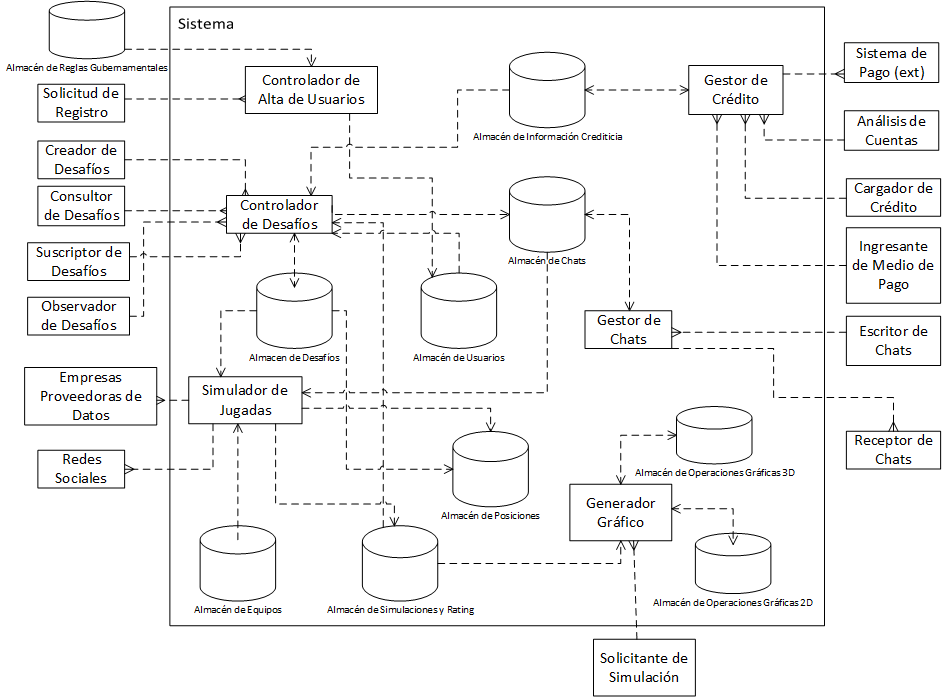
\includegraphics[scale=0.80,angle=90]{diagramas/arquitectura_general}
\label{fig:arquitectura_general}

En la figura \ref{fig:arquitectura_general} se ven los principales componentes del sistema, sobre los cuales se hace zoom en las secciones posteriores, además de los repositorios utilizados para nuestra solución.

\subsection{Controlador de Alta de Usuarios}
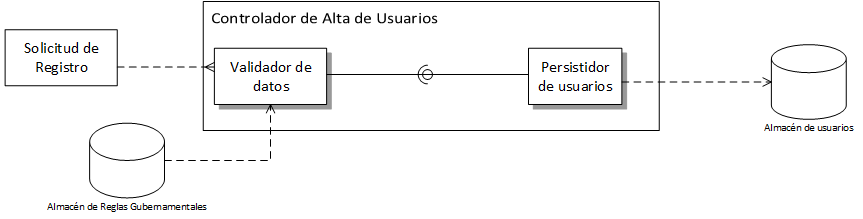
\includegraphics[scale=0.65]{diagramas/controlador_de_usuarios}
\label{fig:controlador_de_usuarios}

Toda solicitud de registro al sistema es recibida por el componente \emph{Controlador de Alta de Usuario}, que consta de tres etapas. 

El \emph{Validador de Datos} es la primera. Tal componente se encarga de validar las distintas posibilidades del usuario con respecto a las reglas gubernamentales establecidas en su país (que se consultan en el repositorio correspondiente). Es, básicamente, un filtro que le permite o no al usuario registrarse de acuerdo a la legislación vigente del territorio desde donde esté entrando al sistema.

Una vez validados los datos, si el usuario incluyó en su registro un método de pago, el \emph{Controlador de Alta de Medios de Pago} validará la información relativa al mismo con el servicio externo correspondiente, y la almacenará en el repositorio adecuado en caso de que sea correcta. El zoom de este componente se verá en la figura \ref{fig:gestor_de_credito}.

Por último, la tercer etapa, el \emph{Persistidor de Usuarios}, es el encargado, ya con todos los datos anteriores validados, de almacenarlos en el repositorio \emph{Almacén de Usuarios}, efectivizando así el registro del usuario.

\newpage
\subsection{Gestor de Crédito}
\begin{center}
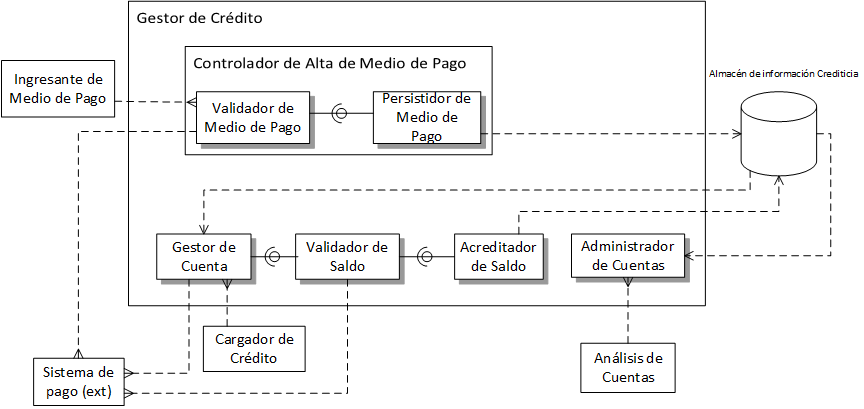
\includegraphics[scale=0.80,angle=90]{diagramas/gestor_de_credito}
\label{fig:gestor_de_credito}
\end{center}

Si un usuario desea pasar del servicio de modalidad gratuita (p.ej., en caso de no haber ingresado un medio de pago a la hora de registrarse) de nuestro sistema al servicio pago, puede realizarlo en cualquier momento (\emph{Ingresante de Medio de Pago}). El componente \emph{Controlador de Alta de Medio de Pago} es el encargado de recibir tales solicitudes, que siempre se encuentran encriptadas.

Este componente cuenta de dos pasos. El primero, \emph{Validador de Medio de Pago}, se encarga de validar la información ingresada comunicándose con el correspondiente servicio de medio de pago externo. El segundo, \emph{Persistidor de Medio de Pago}, es quien -una vez todas las validaciones hayan sido corroboradas y aceptadas- persiste esta información en el \emph{Almacén de Información Crediticia}.

Un usuario puede cargar crédito a su cuenta en cualquier momento (\emph{Cargador de Crédito}). Esta información llega al componente de manera encriptada, y deberá pasar por un pipeline de validaciones, que comienza en el \emph{Gestor de Cuenta}. Este primer paso consta de obtener todos los datos correspondientes a la cuenta, y validar que todavía esté activa. Una vez esta información haya sido confirmada por el \emph{Sistema de Pago (externo)}, el validador de saldo será el encargado de corroborar que la cifra a cargar en cuestión tenga un respaldo en saldo en el medio de pago del usuario (consultando, nuevamente, al \emph{Sistema de Pago (externo)}). Si se confirma esto, el \emph{Acreditador de Saldo} será el que se comunique con el repositorio \emph{Almacén de Información Crediticia} e ingrese el nuevo saldo del usuario.

Cuando un usuario administrador desee consultar los datos de alguna cuenta (\emph{Análisis de Cuentas}), lo hará a través de un componente con privilegios especiales, el \emph{Administrador de Cuenta}, que tiene la capacidad de mostrar y analizar la información crediticia de todos los usuarios. Las comunicaciones con este componente se encuentran también cifradas.

\newpage
\subsection{Gestor de Chats}
\begin{center}
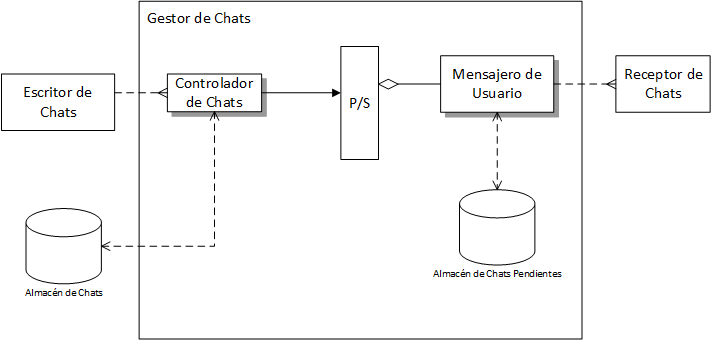
\includegraphics[scale=0.80]{diagramas/gestor_de_chats}
\label{fig:gestor_de_chats}
\end{center}

Los usuarios pueden escribir chats (\emph{Escritor de Chats}) o bien ser quien los recibe (\emph{Receptor de Chats}). Esto ocurre en los distintos tipos de chats que ofrece el sistema, tanto el global del desafío como el individual. 

Quien desee escribirle a otro usuario, se comunicará con el \emph{Controlador de Chats}, quien validará que la persona está disponible para comunicarse en ese chat global en el caso de que sea un chat de desafío, o creará/buscará un chat con el nuevo participante en el caso de los chats individuales. Una vez validada esta información, el componente publicará mediante un conector del tipo \textbf{Publish/Subscribe} la nueva información de chat, y será alguno de los \emph{Mensajero de Usuario} quien se encargará de ponerlo a disponibilidad del receptor. 

Si el usuario receptor no está conectado para recibir el mensaje, el \emph{Mensajero de usuario} cuenta con su propio repositorio (\emph{Almacén de Mensajes Pendientes}, lo que le permite mantener control sobre los mensajes que aún le restan enviar.

\newpage
\subsection{Controlador de Desafíos}
\begin{center}
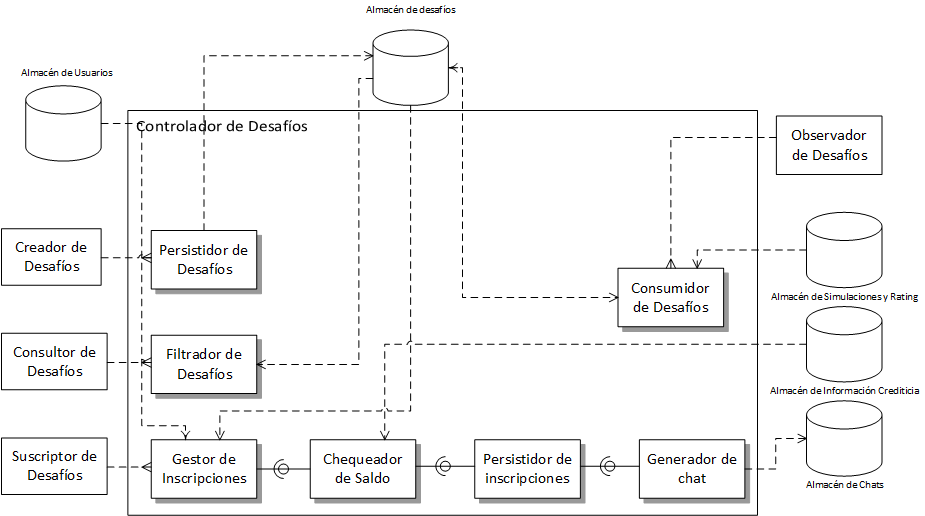
\includegraphics[scale=0.80,angle=90]{diagramas/controlador_de_desafios}
\label{fig:controlador_de_desafios}
\end{center}

El \emph{Controlador de Desafíos} es ya un componente más complejo que el anterior y ofrece diversas interacciones.

Por un lado, el \emph{Creador de Desafíos} se comunica con el \emph{Persistidor de Desafíos} y le comunica sus intenciones de crear un nuevo desafío; el \emph{Persistidor} almacena el nuevo desafío en el \emph{Almacén de Desafíos}, desde donde puede ser consultado por otros de los componentes.

Cuando un usuario desea consultar los desafíos a los que puede inscribirse (\emph{Consultor de Desafíos}), el \emph{Filtro de Desafíos} se encarga de interactuar con los datos del usuario y el \emph{Almacén de Desafíos}, para presentar la información solicitada de manera correcta.

Cuando un usuario desea inscribirse en un desafío (\emph{Suscriptor de Desafíos}), el \emph{Gestor de Inscripciones} es quien recibe la petición con todos los datos del usuario y el desafío en cuestión, y analiza si es posible o no cumplir con el pedido. Si lo es, se le transmite la información al \emph{Chequeador de Saldo}, quien validará -en caso de ser necesario- que el usuario cuente con el saldo suficiente para participar del desafío. 
Estos datos, luego, pasan por un pipe al componente siguiente, quien es el encargado de persistir la información del registro del usuario en el desafío elegido, dejando constancia de la inscripción.
Finalmente, el \emph{Generador de Chat} es quien inscribe al nuevo usuario en el chat global del desafío.

Por otro lado, las noticias y comunicaciones relativas a los desafíos, estén dirigidas a usuarios inscriptos o no, son leídas por el \emph{Consumidor de Desafíos}, quien es el encargado de, a partir de los datos de los desafíos generados y las simulaciones, ofrecer la información correspondiente a quien sigue un desafío (\emph{Seguidor de Desafíos}).


\newpage
\subsection{Simulador de Jugadas}
\begin{center}
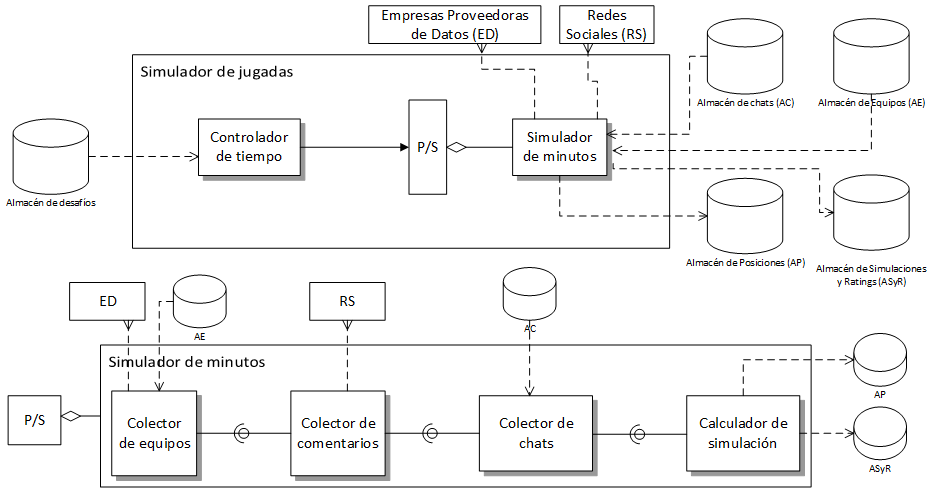
\includegraphics[scale=0.90,angle=90]{diagramas/simulador_de_jugadas}
\label{fig:simulador_de_jugadas}
\end{center}
\newpage
Cada vez que se le dé inicio a un desafío, es el \emph{Controlador de tiempo} del \emph{Simulador de Jugadas} el encargado de publicar la información en un conector de tipo \textbf{Publish/Subscribe}. El \emph{Simulador de Minutos} será quien realice todos los cálculos de la simulación, y los dejará disponibles en el repositorio correspondiente (\emph{Almacén de Simulaciones y Ratings}).

Realizando \emph{zoom} sobre el \emph{Simulador de Minutos}, vemos que se descompone de la siguiente manera:
\begin{itemize}
 \item \emph{Colector de Equipos}: este componente es el encargado de conectarse al \emph{Repositorio de Equipos} y traer la información necesaria de cada uno de los equipos que serán utilizados en la simulación del desafío. La información obtenida es entregada al siguiente componente, el
 \item \emph{Colector de Comentarios}: este componente recorre las distintas redes sociales de forma paralela con el objetivo de procesar la mayor cantidad de comentarios sobre los jugadores de las últimas horas para influir sobre el resultado de la simulación. Obtenida esta información (\textbf{\underline{Nota}}: asumimos que todas las redes sociales cuentan con algún servicio que pueda responder con baja latencia a búsquedas del tipo \'Lionel Messi\'), se enviará por medio de un pipe al siguiente componente en el camino, el
 \item \emph{Colector de Chats}: este componente/conjunto de componentes en paralelo se conecta con el repositorio \emph{Almacén de Chats} para buscar información y comentarios sobre los jugadores, técnicos, etc. de cada uno de los equipos del desafío. Recabada esta información, pasa al siguiente componente,
 \item \emph{Calculador de Simulación}: cuando llegue la información a este componente, la simulación será calculada y persistida en el \emph{Almacén de Simulaciones y Ratings}, junto al desempeño de cada uno de los jugadores participantes en el desafío y, en caso de estar calculando la última jugada del partido, las nuevas posiciones de los participantes en cuestión (persistidas en el \emph{Almacén de Posiciones}).
\end{itemize}


\newpage
\subsection{Generador Gráfico}
\begin{center}
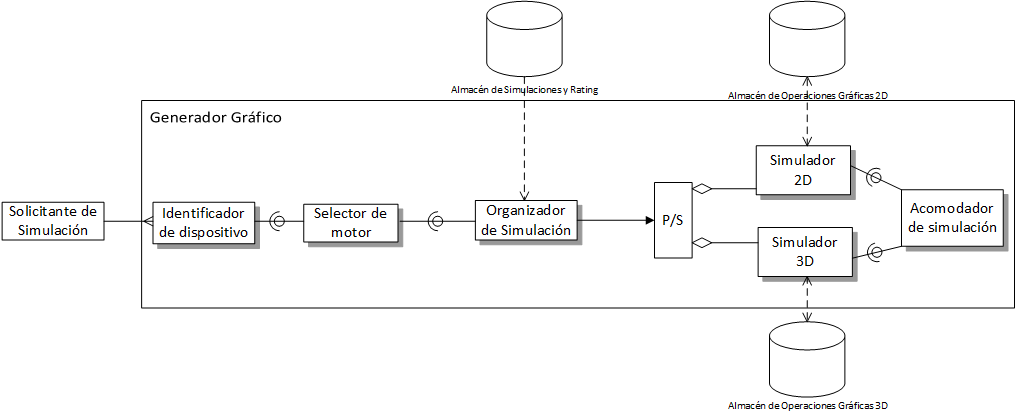
\includegraphics[scale=0.86,angle=90]{diagramas/generador_grafico}
\label{fig:generador_grafico}
\end{center}

Cuando un usuario solicite ver una simulación, será el \emph{Identificador de Dispositivo} el primero en recibir este pedido, y analizar las capacidades gráficas con las que cuenta el aparato en cuestión.

Esta información es enviada al \emph{Selector de Motor}, quien toma la decisión sobre qué motor es el más adecuado (si es que hay uno) para el dispositivo que realizó la solicitud, y envía el resultado mediante un pipe al \emph{Organizador de Simulación}.

Este componente es el encargado de buscar todos los datos necesarios en el repositorio \emph{Almacén de Simulaciones y Ratings}, y publicarlos con un conector Publish/Subscribe junto a la información del motor necesario.

Según el tipo de motor elegido (2D, 3D), el componente adecuado (\emph{Simulador \{2D,3D\}}) lee esa información del Publish/Subscribe, y es el encargado de calcular a partir de los datos recopilados, las instrucciones que reciben los motores gráficos de los dispositivos. Este componente consulta a su propio repositorio (\emph{Almacén de Operaciones Gráficas \{2D,3D\}}), con el fin de tener un caché de aquellos cálculos que se realizan de forma más frecuente. En el caso de que no sea posible utilizar el motor gráfico del dispositivo, un \emph{Motor 3D} en nuestros servidores recibe directamente las instrucciones para la simulación, la genera y la envía al \emph{Streamer}.

Una vez que las instrucciones para los motores (2D, 3D) de la simulación gráfica fueron generadas, este stream de datos que se calcula en tiempo real, será enviado a un último componente, el \emph{Acomodador de Simulación}. La función del mismo es enviar el stream como una serie de paquetes ordenados al dispositivo (de forma parecida al protocolo de sliding window en las conexiones TCP de Internet).


\newpage
\subsection{Streamer}
\begin{center}
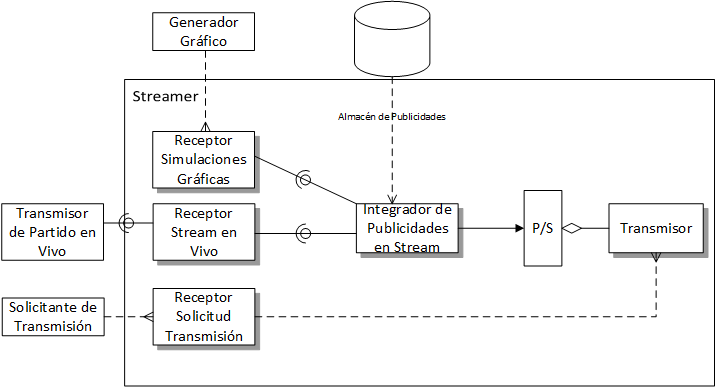
\includegraphics[scale=0.86,angle=90]{diagramas/streamer}
\label{fig:streamer}
\end{center}

El componente \emph{Streamer} es el encargado de realizar la transmisión de video hacia los dispositivos de los usuarios en dos casos, cuando los motores gráficos no soportan al dispositivo en cuestión, o cuando el usuario decidió ver la transmisión de un partido en vivo.

El usuario (\emph{Solicitante de Transmisión}) se comunica con el sistema cuando desea ver un partido en vivo antes de que empiece, y su pedido es recibido por el \emph{Receptor Solicitud de Transmisión}, quien lo reenvía al \emph{Transmisor}. Éste se subscribe al conector \emph{Publish/Subscribe} con el tipo de evento solicitado por el usuario, y queda a la espera de que sea transmitido.

Cuando alguna empresa con los derechos de transmisión de algún partido (\emph{Transmisor de Partido en Vivo}) desea ofrecerlo en nuestra plataforma, se comunica con nuestro sistema y el pedido es recibido por el \emph{Receptor de Stream en Vivo}. El receptor encola este stream en el \emph{Integrador de Publicidades en Stream}. 

Este componente agrega a las transmisiones (ya sean en vivo o simulaciones) las publicidades que se encuentren activas en el repositorio \emph{Almacén de Publicidades}. Luego, se conecta mediante el conector \textbf{Publish/Subscribe} al \emph{Transmisor}, al que le deja disponible el partido con publicidades 
integradas y listo para transmistir al \emph{Solicitante de Transmisión}.

En caso de las simulaciones que no pueden ser generadas en un dispositivo, llega el pedido desde el \emph{Generador Gráfico} al \emph{Receptor de Simulaciones Gráficas}, que encola también el video listo para transmitir en el \emph{Integrador de Publicidades en Stream}.


  \newpage
\section{Arquitectura TP1}
A continuacion detallaremos la arquitectura diseñada en base al enunciado del TP1.

\subsection{Paneo General}
\begin{center}
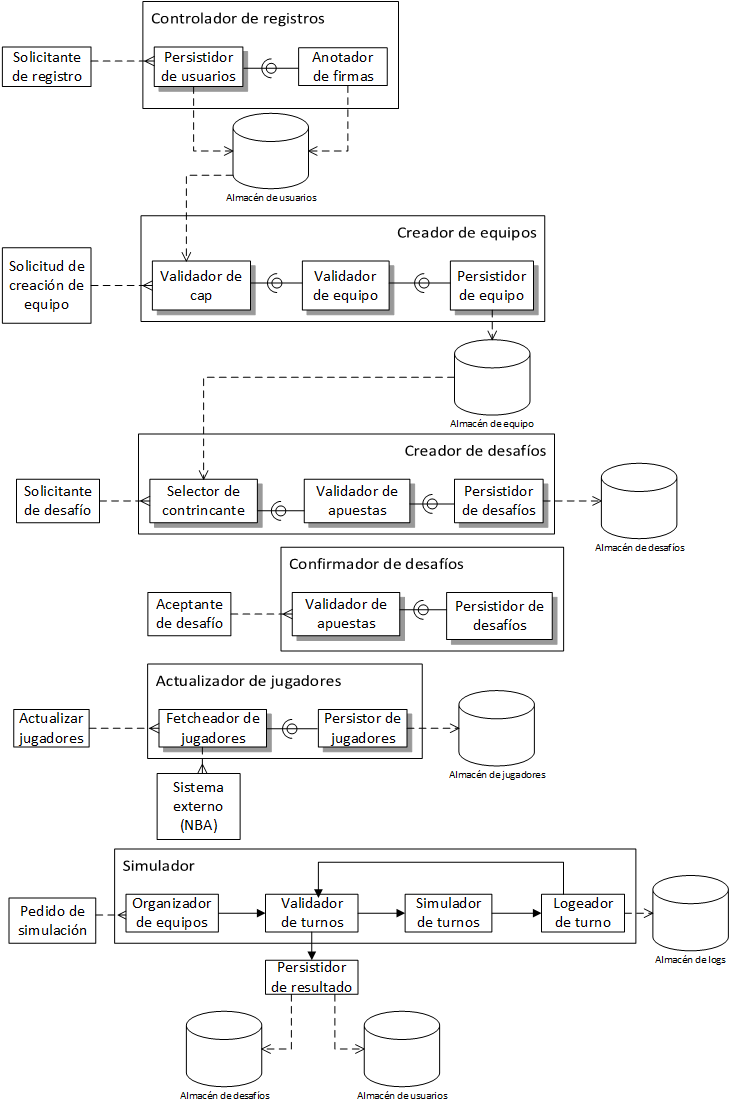
\includegraphics[scale=0.70]{diagramas/tp1/arquitectura_tp1.png}
\end{center}
\label{fig:arquitectura_tp1}

En la figura \ref{fig:arquitectura_tp1} se ven los principales componentes del sistema, sobre los cuales se hace zoom en las secciones posteriores, además de los repositorios utilizados para nuestra solución.

\subsection{Actualizador de jugadores}
\begin{center}
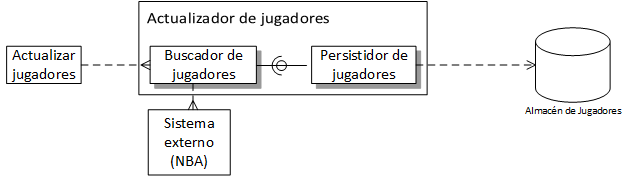
\includegraphics[scale=0.80]{diagramas/tp1/buscadordejugadores.png}
\end{center}
\label{fig:buscadordejugadores}

Dado que existe la posibilidad de actualizar las estadísticas de los jugadores mediante un sistema externo, un administrador podrá realizar esta solicitud que será enviada directamente al \emph{Buscador de jugadores} quien se conectara directamente con el sistema externo para traer la última versión de los datos correspondientes. Esta será enviada directamente al \emph{Persistidor de jugadores} quien actualizara la información de los mismos o agregara nuevos, según sea necesario.

\subsection{Creador y confirmador de desafios}
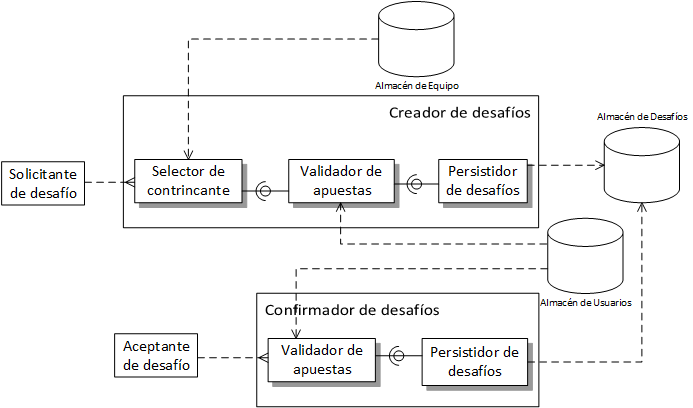
\includegraphics[scale=0.80]{diagramas/tp1/desafios.png}
\label{fig:desafios}

Cuando un usuario solicite desafiar a otro, se enviara la información correspondiente a un componente \emph{Selector de contrincantes} que se encargara de buscar toda la información correspondiente a ambos equipos y la enviara al \emph{Validador de apuestas}. Este último será quien deba confirmar que ambos participantes cuentan con las fichas necesarias (por lo menos en primera instancia), para poder participar del desafío y descontara las fichas necesarias del usuario que solicito el desafío.

Cuando el participante desafiado acepte alguno de los desafíos que se le envían, la comunicación se enviara directamente hacia el \emph{Validador de apuestas}. Este componente validara una vez más que el equipo desafiado cuente con las fichas necesarias (para que no se dé el caso en que, luego de haber sido desafiado, haya gastado sus fichas en otros desafíos) y luego se comunicara con el \emph{Persistidor de desafíos} para que el desafío sea finalmente confirmado, ya por ambas partes.

\subsection{Creador de equipos}
\begin{center}
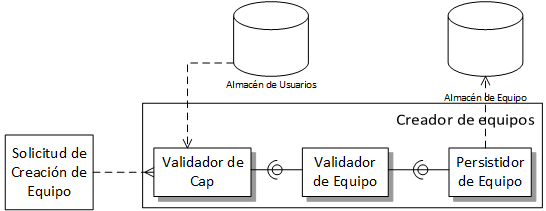
\includegraphics[scale=0.80]{diagramas/tp1/equipo.png}
\end{center}
\label{fig:equipo}

Toda comunicación que se realice con el fin de crear un nuevo equipo, dará inicio a través de un componente \emph{Validador de CAP} que se encargara, mediante la verificacion de los datos almacenados en el repositorio de usuarios, de confirmar que el usuario cuenta con el CAP necesario para poder formar dicho equipo. Un segundo componente (\emph{Validador de equipo}), recibirá la confirmación de este y tendrá como función la de validar la información concreta del equipo (están todas las posiciones ocupadas, jugador estrella elegido, etc.) para luego enviarla al \emph{Persistidor de equipos} que se encargara de almacenarla en el repositorio correspondiente (\emph{Almacén de equipos}).

\subsection{Controlador de registros}
\begin{center}
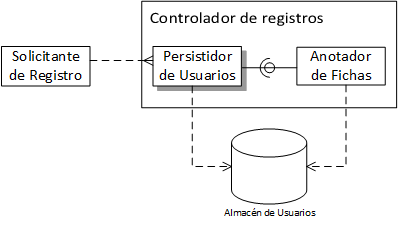
\includegraphics[scale=0.80]{diagramas/tp1/registros.png}
\end{center}
\label{fig:registros}

Toda solicitud de registro de un nuevo usuario es recibida por el \emph{Persistidor de usuarios} encargado de almacenar los datos del mismo en el repositorio \emph{Almacén de usuarios} y envía un mensaje hacia el \emph{Anotador de fichas} que persiste la cantidad de fichas otorgadas al nuevo usuario. El objetivo de mantener estos dos componentes separados es el de ofrecer flexibilidad en el manejo de las fichas y ofrecer la posibilidad de cambiar este módulo con bajo impacto en el sistema.

\subsection{Simulador}
\begin{center}
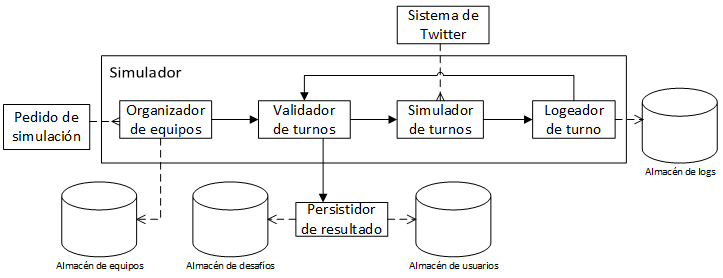
\includegraphics[scale=0.80]{diagramas/tp1/simulador.png}
\end{center}
\label{fig:simulador}

Cuando un nuevo pedido de simulación llegue al sistema, será recibida por un \emph{Organizador de equipos}. Este componente traerá la información de los dos equipos comprometidos en el desafío y se la enviara al \emph{Validador de turnos}. Este componente, que es parte de un ciclo de ejecución, validara que la cantidad de turnos total configurada en el sistema todavía no se haya cumplido y en caso de que todavía haya pendientes, notificara al \emph{Simulador de turnos}. A través de una comunicación directa con el API de Twitter, este componente calculara los resultados de las simulaciones del turno correspondiente. Estas se irán enviando una tras otra hacia el \emph{Logeador  de turnos} que persistirá los datos para que luego estén disponibles para los usuarios. Cuando este componente termine de cumplir su función, notifica una vez más al \emph{Validador de turnos}, para que este revise si todavía quedan pasos por simular. En caso de que esto no sea así, se comunicara con el \emph{Persistidor de resultados}, encargado de almacenar el resultado del desafío y la nueva posición (o el cambio de puntos) de los usuarios participantes.
  \newpage
\section{Conclusiones}
\subsection{Metodologías utilizadas en la materia}
Tanto \textbf{Unified Process} como \textbf{Scrum} son metodologías para el desarrollo de software, que comparten la característica de seguir un modelo iterativo incremental, pero difieren en muchas otras cosas. Aún siguiendo modelos iterativos, por ejemplo, en \textbf{Scrum} cada iteración se planifica cuando termina la anterior, mientras que en \textbf{UP} se planifican todas al comienzo.

\textbf{Scrum} se vende como una metodología ágil con muy poca planificación, lo que la hace por lo tanto muy flexible y adaptable a los cambios y las diferentes circunstancias que vayan surgiendo a medida que se avanza en el desarrollo. Uno de sus pilares, \emph{individuos e interacciones sobre procesos y herramientas}, favorece la comunicación continua entre los programadores y el Project Owner (en forma de Stand Up Meetings), de manera de poder ir resolviendo rápidamente cualquier problema o inquietud que haya surgido. 

Otra máxima de la metodología \textbf{Scrum} es \emph{Software andando sobre documentación exhaustiva}, la cual pone en un lugar de privilegio al cliente, ya que éste valora más tener un software andando a documentación de desarrollo que nunca use y tal vez ni siquiera vea (hay que tener en cuenta, también, que muchas veces el cliente no sabe lo que quiere, por lo que empezar con el producto desde temprano permite que se definan mejor sus requerimientos). Es por esto también que a medida que se planea cada iteración de \textbf{Scrum} (donde están en juego todas las fases de una metodología de desarrollo clásica: requerimiento, análisis, diseño, desarrollo, testing, etc.), se privilegian las \emph{user stories} que le dan más \emph{business value} al cliente. Cada iteración de \textbf{Scrum} (inmodificable; las modificaciones que surjan deberán llevarse a cabo sí o sí en futuras iteraciones) concluye con la presentación de un \emph{entregable}, software ya andando y que debería poder ser puesto en producción, para poder obtener feedback

\textbf{Unified Process}, en cambio, sigue un proceso mucho más estricto guiado por la arquitectura y los casos de uso del software a desarrollar. Consta de 4 fases bien definidas (Inception, Elaboration, Construction y Transition), que se diferencian entre sí según la actividad en la que se haga hincapié (análisis del problema, desarrollo de la solución, etc., por poner dos ejemplos contrapuestos). Este enfoque más estructurado y con foco en la documentación (\emph{conocimiento}) permite ir desarrollando un modelo mental del software a construir e ir entrando en contacto con el problema y las maneras de solucionarlo.

A diferencia de \textbf{Scrum}, en \textbf{UP} el objetivo es en cada iteración ir evitando (o, de ser imposible, reduciendo) los riesgos del sistema a desarrollar, por lo que resulta clave tener un buen entendimiento del dominio del problema -e idealmente, experiencia en él- para ir previendo lo que pueda surgir. Si bien pueden haber entregables en cada etapa de \textbf{UP}, no necesariamente son \textit{código ejecutable}: pueden ser documentos de requerimiento, de análisis de dominio, u otros.

Al tener mucha planificación de entrada, resulta más fácil en \textbf{UP} tener una idea estimada de cuándo finalizará el proyecto, algo que no sucede en \textbf{Scrum} (siempre y cuando, claro, que en UP se hayan estimado bien las cosas, algo que no siempre sucede).

Por lo descrito, \textbf{Scrum} se presenta como una solución ventajosa para proyectos poco críticos y de poca duración, con equipos chicos y sin fechas de finalización estrictas, donde la adaptabilidad y flexibilidad sean importantes para la concreción del desarrollo. Por el enfoque más formal, \textbf{UP} se presenta como una solución ideal para proyectos grandes, complejos, con equipos numerosos, y donde las fechas sean estrictas y jueguen un rol importante.

\newpage
\subsection{Programming in the large \textit{vs} Programming in the small}
La diferencia entre \textbf{programming in the large} y \textbf{programming in the small} parecería desprenderse de la distinción sobre en qué tipo de proyecto es más apto utilizar Scrum o UP. 

\textbf{Programming in the large} consiste en el desarrollo de proyectos de software de gran tamaño, donde están inmersos muchos participantes con requerimientos y necesidades a veces contrapuestos, y durante un período largo de tiempo. Por esa razón conviene un acercamiento estructurado al problema, como el que propone UP, donde conocer los \emph{drivers} del proyecto, las prioridades, los atributos de calidad, tener cronogramas definidos, etc. se vuelve de gran importancia. Descomponer el problema en subsistemas permite que estos puedan ser desarrollados por distintos equipos. 

La arquitectura juega un rol vital en el caso de \textbf{programming in the large}, puesto que permite tener una primera definición de la solución, ver las estructuras del sistema, sus relaciones y propiedades de sus elementos, evitando potenciales problemas posteriores que requieran un cambio mayor en el diseño del sistema y que redunde en un costo muy alto.

\texbtf{Programming in the small} podría ser considerado como el desarrollo de cada uno de los submódulos que componen un sistema mayor. Al estar mucho más circunscripto el alcance de un único módulo, un error puede no ser tan costoso de corregir, por lo que se relajan las tareas de planificación, de análisis de riesgo, y de documentación (pues el sistema es más pequeño y, por lo tanto, más simple de comprender).

\newpage
\subsection{Conclusiones del grupo}
La diferencia conceptual entre los dos TPs de la materia es clara, y esa experiencia es algo que (sentimos que) permea lo que fuimos escribiendo en las últimas dos subsecciones. El primer TP tuvo un enfoque de programming in the small, desarrollando un sistema a pequeña escala y con una metodología bastante particular (justamente por la libertad que ofrece); el segundo TP tuvo un enfoque mucho más estructurado y minucioso, donde no tener un detalle en cuenta al principio ocasionaba una verdadera bola de nieve más adelante (no darle importancia a alguna frase en particular del enunciado puede llevar a cosas importantes y ausentes en la arquitectura final del sistema), por lo que había que ser extremadamente cuidadoso.

Con respecto a UP en sí, más allá de la estructura (en cuanto a cronogramas) y la metodología en sí (las iteraciones, las fases), nos resultaron más interesantes las herramientas utilizadas. Es interesante aprender nuevas herramientas para poder expresar lo que se necesita/espera de un sistema por desarrollar (con los casos de uso, los atributos de calidad, los escenarios como método de desambiguación de los mismos, la arquitectura y todo su lenguaje asociado como primer acercamiento a una solución, etc.), esta expansión de nuestro lenguaje profesional es interesante y nos permitirá en un futuro utilizar las cosas que consideremos útiles del mismo para la realización de nuevos proyectos. Conocer también el estándar de las tácticas es algo importante, para no reinventar la rueda constantemente.

En ninguno de los dos TPs podemos decir que aplicamos la metodología respectiva al 100\%, y ni siquiera un porcentaje algo menor. Seguimos considerando que el tiempo, el ámbito y las circunstancias no son las apropiadas como para poder entrar en calor con ellas y poder ejercer una fuerte opinión sobre sus ventajas y sus desventajas.


  
\end{document}
